% !TEX program = pdflatex
% IEEE conference draft; no venue-specific page limit has been selected.
% The original manuscript is preserved as paper-crewai-original.tex.
% Results refer to the complete 500-by-two study-20261009-v3.
\documentclass[conference]{IEEEtran}
\usepackage[T1]{fontenc}
\usepackage{cite}
\usepackage{amsmath,amssymb}
\usepackage{graphicx}
\usepackage{booktabs}
\usepackage{balance}
\usepackage{array}
\usepackage{url}
\usepackage{xcolor}
\usepackage{tikz}
\usetikzlibrary{arrows.meta,positioning,calc}
\graphicspath{{paper-figures/}}
\newcommand{\NEI}{\textsc{nei}}
\newcommand{\CI}{\textsc{ci}}
\newcommand{\modelname}{\texttt{gemma4:31b-cloud}}
\newcommand{\jevname}{\texttt{jev-1.13.0}}
\newcommand{\pct}{\%}

\begin{document}
\title{KajiAI: Auditable Claim Verification with Bounded Research and Selective Evidence Gates}

% Replace the fields below with the actual authors and affiliations.
\author{\IEEEauthorblockN{Author Name(s)}
\IEEEauthorblockA{\textit{Department and Institution}\\
City, Country\\
Email address or ORCID}}
\maketitle

\begin{abstract}
A correct factual prediction does not necessarily provide verifiable evidence, and additional web research can change a previously correct answer. This paper presents KajiAI, a LangGraph workflow that separates a language model's proposed verdict from an evidence-based acceptance decision. It records versioned retrieved text, checks literal quotation provenance, applies structural evidence requirements and model-based citation review, and repeats research within explicit resource budgets. A completed evaluation assessed all 500 AVeriTeC development claims using both the workflow and a model-only control, retaining 13 execution failures. The workflow achieved 67.4\pct\ label accuracy and 0.500 macro F1, compared with 53.8\pct\ and 0.417 for the control. The paired accuracy difference was 13.6 percentage points, with a 95\pct\ bootstrap interval of 8.6--18.6 points. The complete gate accepted 44 verdicts, of which 42 matched the dataset labels; coverage was 8.8\pct. Additional rounds corrected 18 predictions and changed 25 correct predictions into incorrect outcomes. These results show why prediction quality, acceptance coverage, evidence support and research cost require separate measurement. Contemporary web access, development-set reuse and the absence of independent human citation validation limit the conclusions.
\end{abstract}

\begin{IEEEkeywords}
automated fact-checking, retrieval-augmented generation, LangGraph, citation provenance, selective prediction, AVeriTeC
\end{IEEEkeywords}

\section{Introduction}
Automated fact-checking requires more than assigning a plausibly correct label. A system should identify evidence, connect that evidence to the claim, disclose uncertainty and preserve enough provenance for inspection. FEVER established an evidence-oriented task using claims derived from Wikipedia \cite{fever}. AVeriTeC extends this setting to real-world claims and web evidence \cite{averitec}. Its shared-task score combines verdict correctness with evidence quality \cite{sharedtask}, emphasizing that label agreement alone is an incomplete account of verification.

Retrieval-augmented generation provides external information to a language model \cite{rag}, but retrieved documents, citations and repeated reasoning do not themselves guarantee an evidence-supported verdict. Citation evaluation distinguishes answer correctness from citation quality \cite{alce}. This distinction motivates an architecture in which prediction and acceptance are observable, separate decisions.

We present KajiAI, an auditable workflow implemented with LangGraph. A model proposes a factual label and an evidence assessment. A gate checks retrieved citations, exact quotations, assertion coverage, source-host diversity and domain requirements, followed by automated semantic citation review. Failed checks preserve the prediction while withholding an accepted verdict. Unresolved gaps can trigger further research, subject to limits on rounds, searches, page fetches, elapsed time and reported tokens.

This paper examines three questions: \textbf{RQ1}, how the combined workflow compares with a same-model, model-only control on label prediction; \textbf{RQ2}, which outputs fixed evidence policies select and what label agreement accompanies their coverage; and \textbf{RQ3}, how predictions, acceptance and resource use change across saved research trajectories.

The contribution is an empirical audit of selection and research trajectories in a preserved claim-verification workflow. An explicit state-and-provenance design separates prediction from acceptance, while a frozen, resumable protocol supports failure-inclusive scoring and fixed-evidence policy replay. Together, these records expose where label accuracy, accepted outputs and iteration cost diverge. On 500 development claims, the combined workflow exceeds the model-only control by 13.6 accuracy points; its gate accepts 44 outputs at 8.8\pct\ coverage, of which 42 match gold labels. LangGraph provides the orchestration infrastructure for this empirical audit.

\section{Related Work}
\subsection{Evidence-Based Fact-Checking}
FEVER pairs supported and refuted claims with annotated evidence sentences \cite{fever}. AVeriTeC uses real-world claims, question--answer evidence and textual justifications from web sources \cite{averitec}. The AVeriTeC shared task evaluates evidence retrieval and veracity prediction jointly \cite{sharedtask}. We use its development labels for a local four-class study; our scores are not official AVeriTeC scores and cannot be directly compared with shared-task rankings.

The 2025 AVeriTeC shared task instead specifies open-weight models, a precompiled evidence store, a single-GPU resource constraint and a one-minute processing limit \cite{sharedtask2025}. Our cloud-assisted, contemporary-web protocol does not reproduce those conditions.

\subsection{Retrieval and Citation Evaluation}
RAG combines parametric generation with external document memory \cite{rag}; Self-RAG learns retrieval and critique through reflection tokens \cite{selfrag}. KajiAI instead uses structured assessments, query templates and explicit routing rules, allowing inspection of query generation and stopping behavior.

FIRE integrates retrieval and verification iteratively, choosing a final judgment or another search query using confidence \cite{fire}. EMULATE distributes search-result ranking and webpage-content assessment across agents \cite{emulate}. Iterative research and role separation therefore precede KajiAI. Our empirical focus is preserving source versions, separating provisional prediction from rule-based acceptance, and measuring changes across frozen trajectories.

ALCE evaluates generated answers along fluency, correctness and citation quality dimensions \cite{alce}. Our literal-quote check addresses a narrower property: whether a quoted string occurs in stored text for its cited URL. A separate model reviews whether that quotation supports its attached finding. Neither mechanism independently establishes the truth of the overall verdict.

\subsection{Selective Prediction}
Selective classification trades coverage for accuracy through rejection \cite{selective}. KajiAI selects outputs through evidence requirements; its confidence categories and citation-review scores lack independent calibration, so the reported coverage and conditional label accuracy carry no statistical risk guarantee.

\section{System Design}
\subsection{Stateful Graph and Execution}
LangGraph supports stateful workflows combining deterministic operations and model calls \cite{langgraph}. Eight nodes execute KajiAI's process in Fig.~\ref{fig:architecture}. The shared state includes the original claim, optional reference date, domain, assertions, retrieval ledger, research history, proposed assessment, evidence gaps, budgets and stop reason. Individual claims follow a sequential graph; the study runner processes up to three claims concurrently.

\begin{figure}[t]
\centering
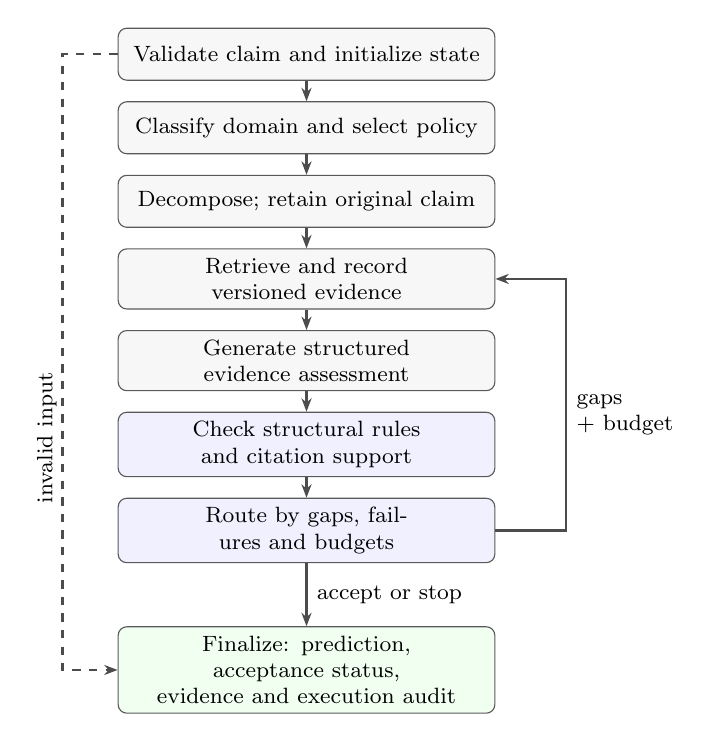
\begin{tikzpicture}[
  node distance=2.6mm,
  flowblock/.style={draw=black!65, rounded corners=1.1mm,
    fill=black!3, align=center, text width=4.55cm,
    minimum height=6.6mm, font=\footnotesize},
  flowgate/.style={flowblock, fill=blue!6},
  flowarrow/.style={-{Stealth[length=1.7mm]}, thick, draw=black!70}
]
\node[flowblock] (validate) {Validate claim and initialize state};
\node[flowblock, below=of validate] (classify) {Classify domain and select policy};
\node[flowblock, below=of classify] (decompose) {Decompose; retain original claim};
\node[flowblock, below=of decompose] (retrieve) {Retrieve and record versioned evidence};
\node[flowblock, below=of retrieve] (analyze) {Generate structured evidence assessment};
\node[flowgate, below=of analyze] (check) {Check structural rules and citation support};
\node[flowgate, below=of check] (route) {Route by gaps, failures and budgets};
\node[flowblock, below=8mm of route, fill=green!6] (finalize)
  {Finalize: prediction, acceptance status,\\evidence and execution audit};
\foreach \from/\to in {validate/classify,classify/decompose,
  decompose/retrieve,retrieve/analyze,analyze/check,check/route}
  \draw[flowarrow] (\from) -- (\to);
\draw[flowarrow] (route) -- node[right, font=\footnotesize] {accept or stop} (finalize);
\draw[flowarrow] (route.east) -- ++(9mm,0)
  |- node[pos=0.23, right, font=\footnotesize, align=left]
  {gaps\\+ budget} (retrieve.east);
\draw[flowarrow, dashed] (validate.west) -- ++(-7mm,0) |-
  node[pos=0.25, left, xshift=-2mm, font=\footnotesize, rotate=90] {invalid input}
  (finalize.west);
\end{tikzpicture}
\caption{Explicit stateful workflow. Remaining gaps can trigger retrieval; failures, stagnation and budgets stop research. Finalization independently rechecks acceptance conditions.}
\label{fig:architecture}
\end{figure}

The evaluated model is \modelname, accessed through a local Ollama endpoint. The cloud model and TinyFish and TypeSafe services make this a network-dependent implementation. Successfully fetched pages are reused within a claim. The study runner resumes at completed claim boundaries; the graph has no persistent checkpoint store.

Jev, accessed through the TypeSafe SDK, supplies the workflow's domain, search-ranking, source-review and citation-support judgments. Domain classification uses Jev when its confidence is at least 0.6, with an Ollama classifier and then keyword scoring as fallbacks. The profiles are general, scientific, political and health/medical. Decomposition is a deterministic conjunction heuristic, limited to six fragments; the original claim is always retained. Fragments are coverage obligations within one assessment, rather than independently executed agents or a weighted verdict ensemble.

\subsection{Query Construction and Retrieval}
At round $t$, retrieval constructs an ordered list from (i) follow-up queries proposed in the previous assessment, (ii) the claim plus \lq\lq evidence,'' (iii) the claim plus \lq\lq counterevidence,'' (iv) each assertion plus \lq\lq evidence,'' and (v) each assertion plus \lq\lq original source fact check.'' It trims and deduplicates strings, excludes previously used queries and selects the first two remaining candidates when the budget permits.

Candidate construction therefore combines model suggestions with hardcoded templates. No learned optimizer chooses the best query. Jev ranks returned URLs for fetching, a separate decision from choosing a query. TinyFish supplies up to five results per search and up to two full-page fetch attempts per search. Failed fetches leave available snippets in the ledger.

A source record stores the URL, query, provider, retrieval time, snippet or page text, content hash and review scores. Full-page text is preferred to a snippet for the same URL, truncated to 20,000 characters and hashed after truncation. The canonical record used in an assessment is retained by URL and hash, permitting replay against the same text version. Jev source review estimates relevance, evidence value, counterevidence value and injection risk. Reviewed records with injection score at least 0.9, or all three relevance/evidence scores below 0.1, are excluded from usable evidence. Unreviewed records retain permissive defaults; this filter is not a demonstrated injection defense.

\subsection{Prediction and Acceptance}
The analyzer returns a structured assessment containing a verdict, confidence category, findings, cited URLs, quotations, assertion resolutions, contradictions, gaps and next queries. It also reports source independence, counterevidence search and, where required, peer-reviewed support. These model-reported flags are policy inputs rather than independently verified facts.

Let $\hat y_i$ be the proposed label for claim $i$, and $G_{s,i}$ and $G_{m,i}$ its structural and semantic gap sets. Acceptance is
\begin{equation}
a_i=\mathbf{1}\{G_{s,i}=\varnothing,\ G_{m,i}=\varnothing,\ F_i=0\},
\label{eq:acceptance}
\end{equation}
where $F_i$ indicates execution failure. The accepted output is
\begin{equation}
\tilde y_i =
\begin{cases}
\hat y_i, & a_i=1,\\
\bot, & a_i=0,
\end{cases}
\label{eq:selective}
\end{equation}
where $\bot$ is operational abstention, not the factual \NEI\ class.

Structural acceptance requires a decisive verdict and High confidence; nonempty retrieved citations for every finding; literal quotations in canonical source text; complete assertion coverage; at least two cited hosts; no flagged duplicate lineage among cited sources; and no unresolved gaps or contradictions. A token-set Jaccard threshold of 0.85 flags substantially similar source text. Counterevidence and independence flags must be positive. Scientific claims require HTTPS citations; health/medical claims require the peer-review flag. A conflicting verdict additionally requires supporting and refuting findings. Established disagreement belongs in those findings and the summary; the contradictions field instead records unresolved objections to the proposed verdict. Distinct hosts, text dissimilarity and model flags do not prove actual independence.

For each eligible finding--URL--quotation triple, Jev reviews the quotation and up to 1,200 surrounding characters on each side. Semantic acceptance requires a \lq\lq supports'' relation with confidence at least 0.8 for every citation. Missing or failed citation checks block acceptance. Review identity includes finding, URL, quotation and content hash; finalization repeats structural checks and confirms review coverage. This tests quotation support for an attached finding, not the entire inferential chain from documents to verdict.

\subsection{Bounded Research and Auditability}
When gaps remain, routing allows further research if execution has not failed and resource and stagnation limits permit it. Two consecutive rounds with no new ledger records trigger a stagnation stop. A new record can be a changed snippet for an already fetched URL, so ledger growth is not equivalent to new usable evidence.

Each round retains its raw assessment, exact usable source versions, gaps, budget snapshot, elapsed time and stop decision. Reported token usage is aggregated, with a completeness flag when accounting is unavailable. Time and token limits govern scheduling; an in-flight request can finish after the soft deadline or exceed the reported-token threshold. Missing usage prevents a guaranteed spend cap. The report preserves proposed and accepted verdicts separately and distinguishes insufficient evidence from execution errors.

\section{Evaluation Protocol}
\subsection{Dataset and Frozen Conditions}
The completed study assesses all 500 AVeriTeC development claims in two conditions. The split contains 122 Supported, 305 Refuted, 35 Not Enough Evidence and 38 Conflicting Evidence/Cherrypicking labels. Only claim text and claim date are supplied as dataset inputs to inference. Gold labels, justifications and annotated evidence are reserved for scoring and post hoc audit. Both conditions use the same model, temperature and structured-output adapter.

The \emph{model-only control} produces one verdict from existing model knowledge without search, domain routing or an evidence gate. The \emph{full workflow} applies the architecture above. Their comparison measures the combined workflow, including its different prompt and evidence context; it does not isolate retrieval, Jev or LangGraph individually. The \emph{first-round analysis} truncates saved full-workflow trajectories rather than constituting a separately executed system.

\begin{table}[t]
\caption{Frozen Evaluation Configuration}
\label{tab:protocol}
\centering
\footnotesize
\begin{tabular}{@{}p{0.38\columnwidth}p{0.55\columnwidth}@{}}
\toprule
Setting & Value\\
\midrule
Main model / temperature & \modelname\ / 0\\
Review model / threshold & \jevname\ / 0.8\\
Research limits per claim & 3 rounds; 300 s soft deadline\\
Search / fetch ceilings & 20 logical searches; 20 fetches\\
Budgeted reported tokens & 250,000 aggregate reported tokens\\
Per-round retrieval & Up to 2 queries; 2 fetches/query\\
Study scheduling & 3 workers; seed 20261009\\
Installed libraries & LangGraph 1.2.11; Pydantic 2.13.5; TypeSafe SDK 0.7.1\\
\bottomrule
\end{tabular}
\end{table}

Table~\ref{tab:protocol} summarizes the protocol. Claim-condition tasks were shuffled with a fixed seed, but contemporary search and cloud-model responses remain externally variable. Source, configuration, package versions, dataset bytes and hashes are archived. Earlier exploratory runs used different source versions and are excluded. Resume checks reject changes to the frozen inference configuration.

The local reproducibility bundle, \texttt{study-20261009-v3}, contains the run manifest, source archive, dataset snapshot, raw JSONL records and per-claim replay results. Source and dataset SHA-256 prefixes are \texttt{624a8d2fa125} and \texttt{499793726b4a}, respectively; the manifest retains their complete hashes. The plotting script reads saved metrics, without issuing additional service calls.

The study retains all 1,000 planned claim-condition attempts, including 8 workflow and 5 control execution failures. A monthly quota limit interrupted execution after 302 workflow and 283 control attempts; seven quota failures remain recorded. Later concurrent-slot timeouts and a local Ollama restart interrupted two pending control requests. Only unattempted tasks were resumed, with the original model, source, dataset and settings; recorded failures were never retried or replaced. Full incident details accompany the reproducibility bundle.

\subsection{Metrics and Uncertainty}
The evaluation schema maps TRUE, FALSE, NOT\_ENOUGH\_EVIDENCE and CONFLICTING to the four dataset labels. Generic MISLEADING predictions are not equated with the conflicting-evidence class. The evidence gate accepts decisive labels only, excluding \NEI\ by design. Accepted \NEI\ recall is therefore zero even when raw predictions are correct.

For $n$ attempted claims and gold labels $y_i$, raw accuracy, coverage and selective accuracy are
\begin{align}
A &= \frac{1}{n}\sum_{i=1}^{n}\mathbf{1}\{\hat y_i=y_i\},\\
C &= \frac{1}{n}\sum_{i=1}^{n}a_i,\\
A_{\mathrm{sel}} &=
\frac{\sum_{i=1}^{n}a_i\mathbf{1}\{\hat y_i=y_i\}}
{\sum_{i=1}^{n}a_i}.
\end{align}
Selective accuracy is undefined when no output is accepted. Macro F1 averages F1 across the four gold classes; abstentions contribute missed predictions without becoming a fifth gold class. End-to-end accepted-label accuracy is $C A_{\mathrm{sel}}$, preventing conditional accuracy from obscuring low coverage.

Fatal errors remain in the denominator. Failure-inclusive scoring treats them as abstentions; raw scoring can preserve an earlier prediction if a later service fails. Raw and failure-inclusive accuracies coincide. We report 95\pct\ Wilson intervals for proportions, a paired accuracy bootstrap with 2,000 claim-level resamples and seed 20261009, and an exact two-sided McNemar test. These intervals treat claims as sampling units; they do not capture correlated topics, shared-source effects, model drift, service availability or web changes.

\subsection{Offline Policy Replay and Citation Audit}
Policy replay applies alternative acceptance rules to the same saved final assessments and source versions. We compare structural-only acceptance with the full gate and semantic thresholds from 0.5 to 0.95. Replay cannot show how changing a gate would alter later retrieval or reasoning. Removing exact-quote requirements also changes eligibility for semantic review, so it is not an isolated semantic ablation.

Citation measurements count finding--URL occurrences in final assessments, including repeated URLs across findings. A blinded human-audit worksheet contains 454 citation rows from 44 accepted and 50 sampled rejected claims; labels and acceptance status are stored separately. Human annotation fields remain blank. Automated Jev judgments are measurements rather than independent human ground truth.

\section{Results}
\subsection{Paired Label Prediction}
Both conditions assess the same 500 claims: 122 Supported, 305 Refuted, 35 \NEI\ and 38 Conflicting labels. Table~\ref{tab:prediction} reports the paired label results, including failed attempts.

\begin{table}[t]
\caption{Prediction Results on All 500 Claims}
\label{tab:prediction}
\centering
\footnotesize
\begin{tabular}{@{}lrrr@{}}
\toprule
Condition & Accuracy (\pct) & 95\pct\ \CI & Macro F1\\
\midrule
Always Refuted & 61.0 & 56.7--65.2 & 0.189\\
Model only & 53.8 & 49.4--58.1 & 0.417\\
First round$^{\dagger}$ & 68.8 & 64.6--72.7 & 0.530\\
Final workflow & 67.4 & 63.2--71.4 & 0.500\\
\bottomrule
\end{tabular}
\par\smallskip
\parbox{\columnwidth}{\footnotesize $^{\dagger}$Saved-trajectory truncation, not a separate live one-round condition. Wilson intervals; local label metrics, not official AVeriTeC evidence scores.}
\end{table}

Full predictions are correct on 337 claims, compared with 269 for the control. The workflow is correct on 117 claims missed by the control, while the control is correct on 49 missed by the workflow; both are correct on 220 and both are wrong on 114. The paired accuracy difference is 13.60 percentage points (bootstrap 95\pct\ \CI: 8.60--18.60); exact McNemar \(p=1.35\times 10^{-7}\).

The majority baseline achieves 61.0\pct\ accuracy because Refuted dominates the split, but its macro F1 is only 0.189. The workflow improves accuracy and macro F1 over the model-only control. It predicts the conflicting class 98 times, compared with 38 gold conflicting labels. Its \NEI\ recall is 17.1\pct, compared with 40.0\pct\ for the control. Improvement is therefore not uniform across classes.

\subsection{Selective Acceptance}
Table~\ref{tab:acceptance} compares acceptance rules on all 500 saved final assessments. Raw prediction accuracy and accepted-label accuracy represent different outcomes.

\begin{table}[t]
\caption{Acceptance Replay on 500 Final Assessments}
\label{tab:acceptance}
\centering
\footnotesize
\begin{tabular}{@{}lrrr@{}}
\toprule
Policy & Accepted & Coverage (\pct) & Correct / accepted\\
\midrule
Structural only & 50 & 10.0 & 45/50 (90.0\pct)\\
Structural + Jev & 44 & 8.8 & 42/44 (95.5\pct)\\
\bottomrule
\end{tabular}
\par\smallskip
\parbox{\columnwidth}{\footnotesize Conditional accuracy 95\pct\ \CI: 78.6--95.7\pct\ for structural-only replay; 84.9--98.7\pct\ for the full gate.}
\end{table}

The full gate withholds 6 outputs accepted by structural-only replay: 3 wrong labels and 3 correct labels. It accepts 35 Refuted, 9 Supported; \NEI\ is excluded by design. Its coverage interval is 6.6--11.6\pct; end-to-end accepted-label accuracy is 8.4\pct. The gate rejects 295 correct raw predictions and 161 wrong ones. Its observed 95.5\pct\ conditional accuracy describes a small selected subset and does not guarantee correct accepted verdicts.

The selected gold labels are 33 Refuted, 9 Supported and 2 Conflicting; the 35 Refuted and 9 Supported counts above describe predictions. On these same 44 IDs, the model-only control matches 30 labels (68.2\pct), while the workflow matches 42. This is a descriptive comparison on a workflow-selected subset, not an independent test of the gate's causal benefit. Selecting only High-confidence assessments instead retains 429 claims with 326 matching labels (76.0\pct); these differently selected cohorts do not establish a calibrated risk guarantee.

Both accepted errors, IDs 353 and 404, have gold conflicting-evidence labels but receive Refuted predictions. In ID 353, the saved assessment uses findings about compensation and legal action to adjudicate a claim specifically about unlicensed vaccines. In ID 404, it combines official denials of complete railway privatization and job losses with reporting about employees' future job-security fears. These illustrative records expose a gap between supporting individual findings and resolving the claim's qualifications and temporal scope. They are case inspections rather than completed human citation annotations.

Figure~\ref{fig:threshold} shows descriptive threshold replay. Stricter thresholds reduce coverage, while lower thresholds can admit additional outputs. Selecting a threshold from this development analysis would require separate validation.

\begin{figure}[t]
\centering
\includegraphics[width=\columnwidth]{acceptance-thresholds.pdf}
\caption{Semantic-threshold replay on 500 final assessments, holding evidence and structural rules fixed. Accepted counts at thresholds 0.50, 0.60, 0.70, 0.80, 0.90 and 0.95 are 46, 45, 44, 44, 30 and 24. The curve does not establish an optimal threshold.}
\label{fig:threshold}
\end{figure}

\subsection{Changes Across Saved Research Rounds}
First-round accuracy is 68.8\pct, compared with 67.4\pct\ for final predictions. Additional rounds change 62 predictions: 18 wrong-to-correct, 25 correct-to-wrong and 19 between incorrect labels. The final-minus-first difference is \(-1.40\) percentage points (bootstrap 95\pct\ \CI: \(-4.00\) to \(1.20\)). Excluding 8 fatal attempts yields \(-0.81\) points on 492 nonfatal attempts, with an interval of \(-3.25\) to \(1.63\).

These saved trajectories quantify within-run changes across later rounds; a separately deployed one-round system can behave differently because timing and search responses can change. Of the attempted workflows, 452 use 3 rounds, 30 use 2 rounds, 18 use 1 round. The prevalence of the round limit warrants evaluating stopping behavior.

Acceptance also changes across the saved trajectories: the first round accepts 14 labels, all matching gold, whereas the final outputs accept 44, with 42 matching gold. Higher final acceptance therefore accompanies lower raw label accuracy in this run. The paired accuracy intervals include zero, so the negative point estimate does not establish an average harmful effect of iteration.

A post hoc query-exhaustion audit identifies 252 third rounds with no additional searches, empty prior follow-up queries and unchanged usable-source versions. These repeated assessments consume 4,154,865 observed tokens. They correct two labels, change one correct label to an incorrect one, and add two acceptances. Truncating those saved rounds would lose one net correct prediction and two acceptances. This motivates testing an explicit stopping policy, while preserving reassessment as a potentially useful operation; it does not demonstrate a cost-only improvement.

\subsection{Citation Diagnostics and Resource Use}
Final assessments contain 2,611 citation occurrences. Of these, 1,914 have literal quotes present in canonical text and 1,914 have Jev reviews. 34 reviewed quotes receive a relation other than \lq\lq supports,'' and 158 receive supporting confidence below 0.8. The remaining 697 occurrences fail literal provenance matching. They are not automatically counted as hallucinations: a quotation can refer to a snippet differing from the preferred full-page text, or exhibit another provenance mismatch.

Final structural gaps include missing exact quotations on 353 claims and insufficient independence flags on 357; these categories overlap. A host-exposure audit unwraps Wayback Machine URLs before comparison. On 208 of 500 claims, a cited host matches the host of the dataset's fact-check article. Host equality does not prove exact-article exposure, and an unmatched host does not exclude other exposure routes.

In the post hoc host-match group, workflow and control accuracies are 77.9\pct\ and 50.5\pct\ (208 claims); in the unmatched group they are 59.9\pct\ and 56.2\pct\ (292 claims). Groups depend on workflow citations and differ in class composition. This is a descriptive exposure audit, not a causal comparison or contamination-free score.

\begin{table}[t]
\caption{Operational Measurements on 500 Tasks per Condition}
\label{tab:cost}
\centering
\footnotesize
\begin{tabular}{@{}lrr@{}}
\toprule
Measurement & Full workflow & Model only\\
\midrule
Attempted tasks & 500 & 500\\
Fatal execution errors & 8 & 5\\
Mean elapsed time (s) & 79.2 & 7.7\\
Median elapsed time (s) & 72.1 & 3.4\\
90th percentile time (s) & 120.1 & 9.0\\
Logical search calls & 2,049 & 0\\
Page-fetch attempts & 3,953 & 0\\
Observed model tokens & 34,452,832 & 183,416\\
\bottomrule
\end{tabular}
\par\smallskip
\parbox{\columnwidth}{\footnotesize Same 500 claim inputs; tokens aggregate providers and accounting is incomplete. Concurrent task durations are not study wall-clock time.}
\end{table}

Table~\ref{tab:cost} reports operational totals. There are 551 recorded fetch failures and 2 Jev ranking failures, distinct from fatal execution errors. The 934 rounds after the first consume 1,049 searches, 2,013 fetch attempts and 23,546,637 observed tokens; 263 add no new ledger records. Incomplete provider-level accounting prevents an exact monetary-cost estimate. Iteration cost and the saved accuracy changes support investigating evidence novelty and stopping rules.

% Balance the final page from its first column.
\subsection{Separate Runtime Development Pilot}
After freezing the historical study, we implemented an opt-in query-exhaustion stop that retains the prior assessment and leaves acceptance rules unchanged. Pending source review or semantic citation gaps preserve reassessment. Focused fixtures reduce provider invocations from three to two (six to four with a repair per assessment), while also demonstrating a possible lost acceptance. The baseline remains the default.

A subsequent authorized live pilot used two development claims (IDs 17 and 246; selection seed 20261102), both conditions, the same model and historical configuration, with shared tighter output limits and disabled service retries. A structured-output smoke passed. Actual use was 11 Ollama, 31 Jev, 11 search and 22 fetch requests: 75 in total. Transport records report 190,142 Ollama and 79,658 Jev tokens, including the smoke and failed attempt; these are observed usage, not monetary costs. One baseline failed because of a local UTF-8 logging defect. Its failure was retained; after repair and verification of complete responses, only unstarted conditions continued within the original budget. Three workflows completed; all predicted Refuted and none passed the evidence gate. Both candidate trajectories exhausted queries after round two, but semantic citation gaps kept the conservative guard active, so neither stopped early. The one complete pair used three model assessments per condition. This pilot is inconclusive about stopping benefit and supports no efficacy claim or full-study launch. Human citation validation remains outstanding.

\balance
\section{Discussion and Limitations}
\subsection{What the Results Support}
The paired comparison shows higher label accuracy for this combined workflow than for its control. Semantic replay withholds both correct and incorrect labels; saved trajectories expose costly reassessment with mixed prediction changes. Prediction, acceptance and resource use therefore warrant separate measurement.

The study includes no independently executed retrieval-only, Jev-disabled or alternative-framework comparison. Its evidence supports neither framework superiority, a hallucination-reduction percentage nor benchmark-leading performance.

\subsection{Threats to Validity}
\textit{Service availability:} In the historical 500-claim study, all planned claim-condition attempts are complete, including 13 recorded fatal failures. Quota and concurrent-slot interruptions required resumption across time. A post hoc sensitivity analysis on 487 pairs without fatal errors gives a workflow-minus-control difference of 14.37 points (bootstrap 95\pct\ \CI: 9.45--19.10); remote responses and current web results can drift. Retaining failures exposes operational performance, while rerunning failed claims and silently replacing them would change the experiment.

\textit{Temporal and verdict exposure:} Retrieval uses the contemporary web without a historical publication cutoff. Later reports and published verdicts can help predict older claims. Original AVeriTeC annotations address temporal evidence concerns \cite{averitec}, but our protocol does not reproduce that constraint. Pretraining exposure is unknown, and the repeatedly used development split is not a pristine held-out test.

\textit{Evidence validity:} Literal checks verify provenance only. Jev support judgments lack independent calibration and human entailment labels. Model-reported independence and peer-review flags can be wrong. Text similarity can miss paraphrased copying or flag legitimate overlap; snippets can omit qualifying context. The prepared human audit has not been performed.

\textit{Task and control scope:} Different prompts make the model-only comparison a combined-workflow effect. Heuristic decomposition can create incomplete fragments. Excluding \NEI\ from acceptance restricts task coverage. Multilingual, multimodal, adversarial and user-facing behavior has not been evaluated.

\textit{Reproducibility:} Hashes preserve source and text, not future service responses. Temperature zero does not guarantee bitwise reproducibility. Soft deadlines, incomplete token accounting and quotas affect measurements. Hosted model revisions and complete provider-specific response metadata were not preserved and cannot be reconstructed. Secrets are excluded from archived artifacts.

\subsection{Next Evaluation Steps}
Independent human review should assess citation support and source credibility, retaining separate annotations and adjudication for the accepted and rejected strata. A targeted follow-up should distinguish exhausted states with completed citation review from those requiring semantic reassessment, before any larger stopping-policy study. The bounded pilot above did not establish a resource benefit. A separate study can compare one-round and iterative workflows under controlled retrieval. A held-out, temporally constrained evaluation and independently executed retrieval-only and Jev-disabled conditions would better isolate the contribution of each mechanism. Such changes must be versioned and evaluated separately to avoid mixing post hoc improvements into this condition.

\section{Conclusion}
KajiAI makes proposed verdicts, evidence acceptance and research history independently inspectable. In a completed 500-claim AVeriTeC development evaluation, the workflow improves paired label accuracy over a model-only control, while a strict gate accepts few claims and later research can worsen saved predictions. The measured tradeoff concerns coverage, conditional label agreement and cost: higher final acceptance accompanies lower raw prediction accuracy across the saved trajectories.

\section*{Acknowledgment}
OpenAI Codex assisted with drafting Sections I--VII, creating the architecture diagram and data-driven plotting code, and auditing evaluation scripts and regression tests. Numerical results were computed from saved execution records. Independent human citation validation was not performed. The authors are responsible for reviewing the manuscript, sources and findings before submission.

\begin{thebibliography}{10}
\bibitem{fever}
J. Thorne, A. Vlachos, C. Christodoulopoulos, and A. Mittal, \lq\lq FEVER: A large-scale dataset for fact extraction and verification,'' in \emph{Proc. NAACL-HLT}, vol. 1, 2018, pp. 809--819, doi: 10.18653/v1/N18-1074.

\bibitem{averitec}
M. Schlichtkrull, Z. Guo, and A. Vlachos, \lq\lq AVeriTeC: A dataset for real-world claim verification with evidence from the web,'' in \emph{Advances in Neural Information Processing Systems}, vol. 36, 2023. [Online]. Available: \url{https://arxiv.org/abs/2305.13117}

\bibitem{sharedtask}
M. Schlichtkrull et al., \lq\lq The Automated Verification of Textual Claims (AVeriTeC) shared task,'' in \emph{Proc. Seventh Fact Extraction and VERification Workshop}, 2024, pp. 1--26, doi: 10.18653/v1/2024.fever-1.1.

\bibitem{rag}
P. Lewis et al., \lq\lq Retrieval-augmented generation for knowledge-intensive NLP tasks,'' in \emph{Advances in Neural Information Processing Systems}, vol. 33, 2020. [Online]. Available: \url{https://arxiv.org/abs/2005.11401}

\bibitem{alce}
T. Gao, H. Yen, J. Yu, and D. Chen, \lq\lq Enabling large language models to generate text with citations,'' in \emph{Proc. EMNLP}, 2023, pp. 6465--6488, doi: 10.18653/v1/2023.emnlp-main.398.

\bibitem{sharedtask2025}
M. Akhtar et al., \lq\lq The 2nd Automated Verification of Textual Claims (AVeriTeC) shared task: Open-weights, reproducible and efficient systems,'' in \emph{Proc. Eighth Fact Extraction and VERification Workshop}, 2025, pp. 201--223, doi: 10.18653/v1/2025.fever-1.15.

\bibitem{selfrag}
A. Asai, Z. Wu, Y. Wang, A. Sil, and H. Hajishirzi, \lq\lq Self-RAG: Learning to retrieve, generate, and critique through self-reflection,'' in \emph{Proc. International Conference on Learning Representations}, 2024. [Online]. Available: \url{https://arxiv.org/abs/2310.11511}

\bibitem{fire}
Z. Xie et al., \lq\lq FIRE: Fact-checking with iterative retrieval and verification,'' in \emph{Findings of the Association for Computational Linguistics: NAACL 2025}, 2025, pp. 2901--2914, doi: 10.18653/v1/2025.findings-naacl.158.

\bibitem{emulate}
S. Hong, M. Luo, and X. Wan, \lq\lq EMULATE: A multi-agent framework for determining the veracity of atomic claims by emulating human actions,'' in \emph{Proc. Eighth Fact Extraction and VERification Workshop}, 2025, pp. 179--183, doi: 10.18653/v1/2025.fever-1.13.

\bibitem{selective}
Y. Geifman and R. El-Yaniv, \lq\lq Selective classification for deep neural networks,'' in \emph{Advances in Neural Information Processing Systems}, vol. 30, 2017. [Online]. Available: \url{https://arxiv.org/abs/1705.08500}

\bibitem{langgraph}
LangChain, \lq\lq LangGraph overview.'' Accessed: Oct. 10, 2026. [Online]. Available: \url{https://docs.langchain.com/oss/python/langgraph/overview}
\end{thebibliography}
\end{document}

